\section{Cortex-M Architecture}

\begin{concept}{Core Architecture Overview}\\
The ARM Cortex-M is a 32-bit processor architecture designed for embedded systems:
\begin{itemize}
  \item Load/store architecture
  \item 32-bit data path
  \item Thumb instruction set
  \item Hardware multiply and optional divide
  \item Harvard architecture variant \\(separate instruction and data buses)
  \item Designed for embedded applications:
    \begin{itemize}
      \item Low cost and power consumption
      \item Real-time capabilities
      \item Interrupt handling
      \item Debug support
    \end{itemize}
\end{itemize}
\end{concept}

\begin{definition}{Registers}\\
The Cortex-M has 16 core registers, each 32-bit wide:

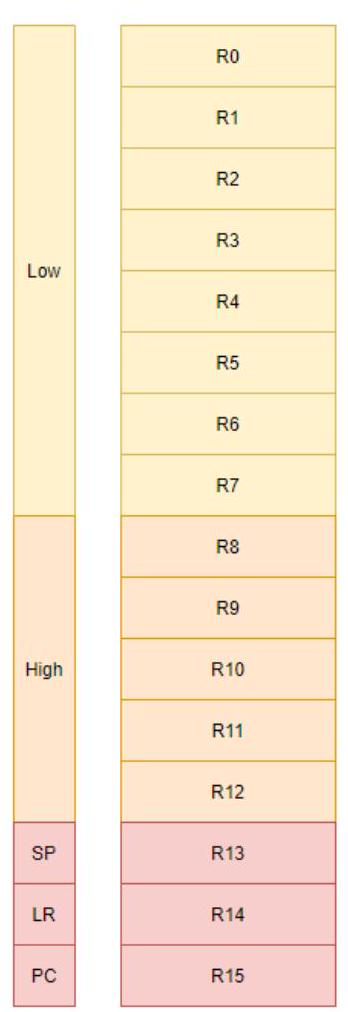
\includegraphics[width=0.35\linewidth, angle=90]{images/2024_12_29_79e6b22f503fb7b4f718g-02}
\begin{itemize}
  \item \textcolor{darkcorn}{\textbf{R0-R7}}: Lower registers - general purpose
    \begin{itemize}
      \item Used by most instructions
      \item Parameter passing in functions (R0-R3)
      \item Results returned in R0
    \end{itemize}
  \item \textcolor{darkorange}{\textbf{R8-R12}}: Higher registers - general purpose
    \begin{itemize}
      \item Limited instruction support
      \item Often used for temporary storage
    \end{itemize}
  \item \textcolor{darkred}{\textbf{R13 (SP)}}: \textcolor{darkred}{\textbf{S}}tack \textcolor{darkred}{\textbf{P}}ointer - temporary storage
    \begin{itemize}
      \item Points to current stack position
      \item Must be word-aligned (multiple of 4)
    \end{itemize}
  \item \textcolor{darkred}{\textbf{R14 (LR)}}: \textcolor{darkred}{\textbf{L}}ink \textcolor{darkred}{\textbf{R}}egister - return address from procedures
    \begin{itemize}
      \item Stores return address for function calls
      \item Can be saved to stack for nested calls
    \end{itemize}
  \item \textcolor{darkred}{\textbf{R15 (PC)}}: \textcolor{darkred}{\textbf{P}}rogram \textcolor{darkred}{\textbf{C}}ounter - address of next instruction
    \begin{itemize}
      \item Points to next instruction
      \item Auto-incremented during execution
    \end{itemize}
\end{itemize}
\end{definition}

\begin{definition}{Arithmetic Logic Unit (ALU)}\\
32-bit wide processing Unit and supports:
\begin{itemize}
  \item Arithmetic operations:
    \begin{itemize}
      \item Addition (ADD, ADC)
      \item Subtraction (SUB, SBC)
      \item Multiplication (MUL)
      \item Division (Optional)
    \end{itemize}
  \item Logic operations:
    \begin{itemize}
      \item AND, ORR, EOR (XOR)
      \item BIC (Bit Clear)
      \item MVN (NOT)
    \end{itemize}
  \item Shift and rotate operations
  \item Compare operations
\end{itemize}
\end{definition}

\begin{definition}{APSR (Flag Register)}\\
The Application Program Status Register (APSR) contains flags:
\begin{itemize}
  \item \textbf{N}: Set when result is negative (bit 31 = 1)
  \item \textbf{Z}: Set when result is zero
  \item \textbf{C}: Set on carry or borrow
  \item \textbf{V}: Set on signed overflow
\end{itemize}

Instruction suffix 'S' (e.g., ADDS) updates these flags.
\end{definition}

\begin{example2}{Flag Usage Examples}\\
After arithmetic operations with 'S' suffix:
\begin{lstlisting}[language=armasm, style=basesmol]
MOVS    R0, #0xFF    ; R0 = 255 (max unsigned 8-bit)
ADDS    R0, #1       ; R0 = 0, Z=1, C=1 (overflow)

MOVS    R0, #0x7F    ; R0 = 127 (max signed 8-bit)
ADDS    R0, #1 ; R0 = 128, N=1, V=1 (signed overflow)

MOVS    R0, #5
SUBS    R0, #10      ; R0 = -5, N=1, C=0 (borrow)
\end{lstlisting}
\end{example2}

\begin{definition}{Instruction Set}\\
The Cortex-M uses 16-bit Thumb instructions:

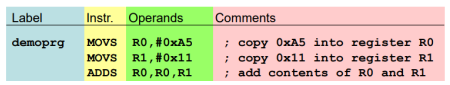
\includegraphics[width=\linewidth]{images/instruction_set.png}

Main instruction types:
\begin{itemize}
  \item \textbf{Data Transfer}: Move, Load, Store operations
    \begin{itemize}
      \item MOV/MOVS - Register to register
      \item LDR/STR - Memory access
      \item PUSH/POP - Stack operations
      \item LDM/STM - Multiple register transfer
    \end{itemize}
  \item \textbf{Data Processing}: Arithmetic, logical, shift operations
    \begin{itemize}
      \item ADD/SUB - Arithmetic
      \item AND/ORR/EOR - Logical
      \item LSL/LSR/ASR - Shifts
      \item CMP/CMN - Compare
    \end{itemize}
  \item \textbf{Control Flow}: Branch and function calls
    \begin{itemize}
      \item B - Branch
      \item BL - Branch with Link
      \item BX - Branch and Exchange
      \item Conditional variants (BEQ, BNE, etc.)
    \end{itemize}
\end{itemize}
\end{definition}



\begin{example2}{Common Instruction Formats}\\
Register operations:
\begin{lstlisting}[language=armasm, style=basesmol]
; Register operations
ADDS    R0, R1, R2   ; R0 = R1 + R2
MOVS    R0, R1       ; R0 = R1
ANDS    R0, R1       ; R0 = R0 & R1
; Immediate values
MOVS    R0, #100     ; Load immediate value
ADDS    R0, R0, #1   ; Add immediate
CMP     R0, #10      ; Compare with immediate
; Memory access
LDR     R0, [R1]     ; Load from memory
STR     R0, [R1, #4] ; Store with offset
LDRB    R0, [R1]     ; Load byte
\end{lstlisting}
\end{example2}

\begin{code}{Basic Assembly Program Structure}
Example of a simple assembly program:
\begin{lstlisting}[language=armasm, style=basesmol]
Label   Instr.  Operands   Comments
demoprg MOVS    R0,#0xA5   ;copy 0xA5 into R0
        MOVS    R1,#0x11   ;copy 0x11 into R1
        ADDS    R0,R0,R1   ;add R0 and R1, store in R0
\end{lstlisting}
\end{code}

\begin{concept}{Assembly Program Sections}
Program memory organized in sections:

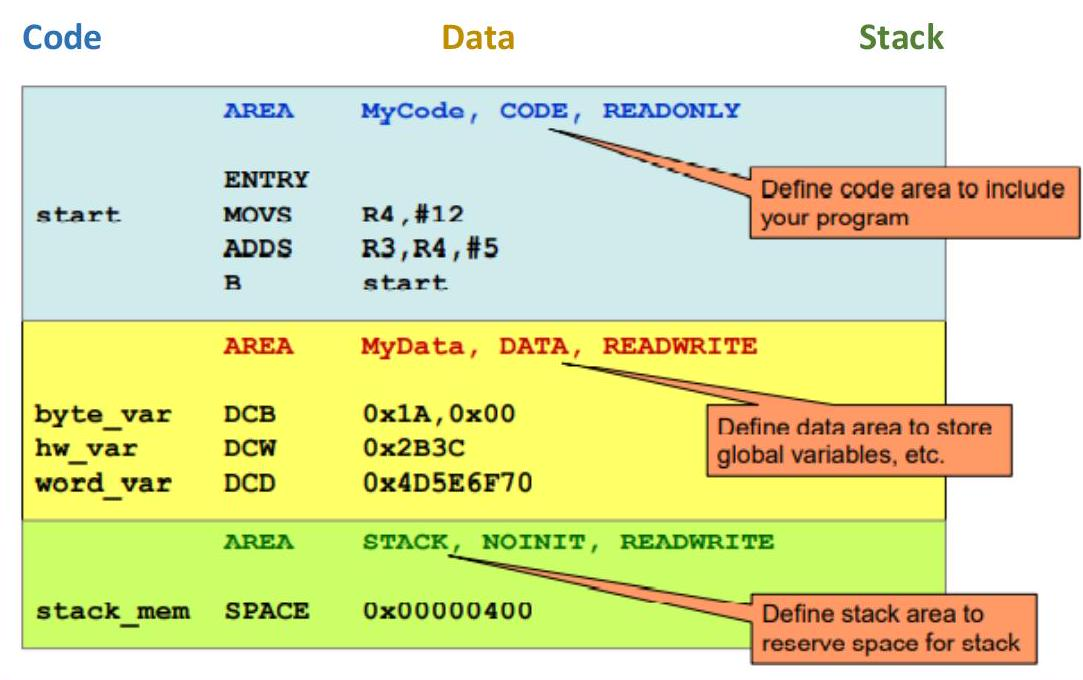
\includegraphics[width=\linewidth]{images/2024_12_29_79e6b22f503fb7b4f718g-02(1)}

\begin{minipage}[t]{0.5\linewidth}
\textcolor{darkblue}{\textbf{Code Section (CODE):}}
\begin{itemize}
  \item Contains program instructions
  \item Usually read-only
  \item Placed in Flash memory
  \item Can contain constants \\(literal pool)
\end{itemize}
\end{minipage}
\begin{minipage}[t]{0.5\linewidth}
\textcolor{darktangerine}{\textbf{Data Section (DATA):}}
\begin{itemize}
  \item Contains global/static variables
  \item Read-write access
  \item Placed in RAM
  \item Initialized at startup
\end{itemize}
\end{minipage}
\vspace{2mm}\\
\textcolor{darkfrog}{\textbf{Stack Section: (STACK)}}
\begin{itemize}
  \item Dynamic memory allocation
  \item Used for local variables
  \item Function call management
  \item Grows downward in memory
\end{itemize}
\end{concept}

\begin{concept}{Initialized vs uninitialized Data}
 
\begin{minipage}{0.75\linewidth}
\textbf{Directives for initialized data:}
\begin{itemize}
  \item \textbf{DCB}: Define Constant Byte (8-bit)
  \item \textbf{DCW}: Define Constant Half-Word (16-bit)
  \item \textbf{DCD}: Define Constant Word (32-bit)
\end{itemize}
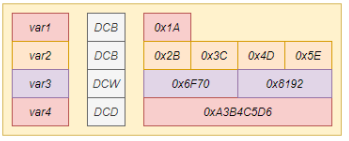
\includegraphics[width=\linewidth]{images/init_data.png}

\textbf{Directive for uninitialized data:}
\begin{itemize}
  \item \textbf{SPACE}: Reserve specified number of bytes
\end{itemize}
\end{minipage}
\hspace{2mm}
\begin{minipage}{0.15\linewidth}
  \vspace{-15mm}
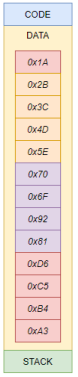
\includegraphics[width=\linewidth]{images/uninit_data.png}
\end{minipage}  
\end{concept}

\begin{code}{Data Definition}
Memory layout for different data types:
\begin{lstlisting}[language=armasm, style=basesmol]
var1    DCB     0x1A                ;single byte
var2    DCB     0x2B,0x3C,0x4D,0x5E ;byte array
var3    DCW     0x6F70,0x8192       ;half-words
var4    DCD     0xA3B4C5D6          ;word
data    SPACE   100                 ;reserve 100 bytes
\end{lstlisting}
\end{code}

\begin{KR}{Creating Assembly Programs}
Steps for creating an assembly program:

1. Define program sections: (CODE, DATA)
\begin{lstlisting}[language=armasm, style=basesmol]
    AREA    |.text|, CODE, READONLY
    AREA    |.data|, DATA, READWRITE
\end{lstlisting}

2. Declare external symbols: (IMPORT/EXPORT)
\begin{lstlisting}[language=armasm, style=basesmol]
    IMPORT  external_func    ; External function
    EXPORT  my_function     ; Public function
\end{lstlisting}

3. Define data:
\begin{itemize}
  \item Define initialized data using DCx directives
  \item Reserve uninitialized data using SPACE
\end{itemize}
\begin{lstlisting}[language=armasm, style=basesmol]
    AREA    |.data|, DATA, READWRITE
var1    DCD     0x1234        ; Word
array   SPACE   100          ; Reserve space
\end{lstlisting}

4. Write program code using proper instruction syntax:
\begin{lstlisting}[language=armasm, style=basesmol]
    AREA    |.text|, CODE, READONLY
    ENTRY                   ; Program entry
main
    ; Your code here
    END
\end{lstlisting}

5. End program with END directive!
\end{KR}





\begin{code}{Common Assembly Patterns}\\
1. Loop with counter:
\begin{lstlisting}[language=armasm, style=basesmol]
    MOVS    R0, #0          ; Initialize counter
loop  ; Loop body
    ADDS    R0, #1          ; Increment
    CMP     R0, #10         ; Check condition
    BLT     loop           ; Branch if less than
\end{lstlisting}

2. Memory copy:
\begin{lstlisting}[language=armasm, style=basesmol]
    ; R0 = source, R1 = destination, R2 = count
copy_loop
    LDR     R3, [R0], #4    ; Load and increment
    STR     R3, [R1], #4    ; Store and increment
    SUBS    R2, #1          ; Decrement counter
    BNE     copy_loop      ; Continue if not done
\end{lstlisting}

3. Function call with parameters:
\begin{lstlisting}[language=armasm, style=basesmol]
    MOVS    R0, #1          ; First parameter
    MOVS    R1, #2          ; Second parameter
    BL      function        ; Call function
    ; Result in R0
\end{lstlisting}
\end{code}

\begin{example2}{Complete Program Example}\\
  %TODO: better example
Program to sum array elements:
\begin{lstlisting}[language=armasm, style=basesmol]
    AREA    |.text|, CODE, READONLY
    EXPORT  array_sum
        
array_sum
    MOVS    R2, #0          ; Initialize sum
    MOVS    R3, #0          ; Initialize index
loop
    LDR     R1, [R0, R3]    ; Load array element
    ADDS    R2, R2, R1      ; Add to sum
    ADDS    R3, R3, #4      ; Next element
    CMP     R3, #16         ; Check if done
    BLT     loop           ; Continue if not
    MOVS    R0, R2          ; Return sum
    BX      LR             ; Return
    END
\end{lstlisting}
\end{example2}




